\section{Results and discussions}
\label{section:results_and_discussions}
%%%%%%%%%%%%%%%%%%%%%%%%%%%%%%%%%%%%%%%%%%%%%%%%%%%%%%%%%%%%%%%%%%%%%%%%%%%%%%%%
In this section, five DL models  of semantic segmentation approach including  Res-UNet, VGG16 encoder-decoder, FCN-DenseNet, PSPNet and GCN were evaluated on exemplary three damage scenarios of an RMS of the full wavefield interpolated at the bottom surface of the plate (numerically generated) in order to identify the delamination.
Additionally, an experimental scenario was also used to evaluate the performance of the models to show the DL capabilities of generalization.
For each model, the mean and the max \(IoU\) are calculated and presented as a metric of comparison.
Moreover, the Accuracy of classification, Precision, Recall, and F1-score depicted in Eqs~(\ref{accuracy}-\ref{f1_score}) respectively, were calculated for each model.
\begin{equation}
	\rm Accuracy\ = \frac{TP+TN}{(Total\ number\ of\ tested\ samples)}
	\label{accuracy}
\end{equation}

\begin{equation}
	\rm Pricision\ =\frac{TP}{TP+FP}
	\label{pricisoin}
\end{equation}
\begin{equation}
	\rm Recall\ = \frac{TP}{TP+ FN}
	\label{recall}
\end{equation}
\begin{equation}
	\rm F1-Score =\frac{2 \times (Pricision\times Recall)}{(Pricision + Recall)} 
	\label{f1_score}
\end{equation}
where the Positive/Negative refers to the predicted output as (damage or non-damage) respectively, True Positive (TP) and True Negative (TN)  represent the correct classification, and the False Positive (FP) and False Negative (FN) represent the incorrect classification.

In our work, all semantic segmentation models were implemented and trained with Keras API~\cite{chollet2015keras} (an open-source platform) running on top of TensorFlow on an NVIDIA Tesla V100 GPU. 
Moreover, for training purposes, we have used K-fold CV technique with \(k=5\). Accordingly, each model has been trained for \(5\) iterations, then the mean accuracy of all folds is calculated. 
Further, for each iteration, the models were trained on the augmented dataset up to \(20\) epochs.
%%%%%%%%%%%%%%%%%%%%%%%%%%%%%%%%%%%%%%%%%%%%%%%%%%%%%%%%%%%%%%%%%%%%%%%%%%%%%%%%

The first exemplary delamination scenario is shown in Fig.~\ref{fig:softmax_448}. 
The delamination is located at the left edge of the plate and its corresponding ground truth image are shown in Fig.~\ref{fig:RMS_flat_shell_Vz_448} and ~\ref{fig:m1_rand_single_delam_448} respectively. 
Figures~\ref{fig:unet_pred_448} -~\ref{fig:gcn_pred_448} show the predicted output of the Res-UNet, VGG16 encoder-decoder, PSPNet, FCN-DenseNet and GCN models, respectively. 
%%%%%%%%%%%%%%%%%%%%%%%%%%%%%%%%%%%%%%%%%%%%%%%%%%%%%%%%%%%%%%%%%%%%%%%%%%%%%%%%
\begin{figure} [!h]
	\centering
	\begin{subfigure}[b]{0.47\textwidth}
		\centering
		\includegraphics[scale=1.0]{RMS_flat_shell_Vz_448_500x500bottom.png}
		\caption{RMS bottom}
		\label{fig:RMS_flat_shell_Vz_448}
	\end{subfigure}
	\hfill
	\begin{subfigure}[b]{0.47\textwidth}
		\centering
		\includegraphics[scale=1.0]{m1_rand_single_delam_448.png}
		\caption{Ground truth}
		\label{fig:m1_rand_single_delam_448}
	\end{subfigure}
	\begin{subfigure}[b]{0.47\textwidth}
		\centering
		\includegraphics[scale=1.0]{residual_unet_num_269.png}
		\caption{Res-UNet}
		\label{fig:unet_pred_448}
	\end{subfigure}
	\hfill
	\begin{subfigure}[b]{0.47\textwidth}
		\centering
		\includegraphics[scale=1.0]{VGG16_ecoder_decoder_num_269.png}
		\caption{VGG16 encoder-decoder}
		\label{fig:vgg16_pred_448}
	\end{subfigure}
	\hfill
	\begin{subfigure}[b]{0.47\textwidth}
		\centering
		\includegraphics[scale=1.0]{PSPNet_num_269.png}
		\caption{PSPNet}
		\label{fig:pspnet_pred_448}
	\end{subfigure}
	\hfill
	\begin{subfigure}[b]{0.47\textwidth}
		\centering
		\includegraphics[scale=1.0]{FCN_DenseNet_num_269.png}
		\caption{FCN-DenseNet}
		\label{fig:fcn_densenet_pred_448}
	\end{subfigure}
	\hfill
	\begin{subfigure}[b]{0.47\textwidth}
		\centering
		\includegraphics[scale=1.0]{GCN_num_269.png}
		\caption{GCN}
		\label{fig:gcn_pred_448}
	\end{subfigure}

	\caption{First damage scenario}
	\label{fig:softmax_448}
\end{figure} 
\clearpage
%%%%%%%%%%%%%%%%%%%%%%%%%%%%%%%%%%%%%%%%%%%%%%%%%%%%%%%%%%%%%%%%%%%%%%%%%%%%%%%%
In the second delamination scenario as shown in Fig.~\ref{fig:385_softmax}, the delamination is located at the upper left corner of the plate and its corresponding ground truth image are shown in Fig.~\ref{fig:RMS_flat_shell_Vz_385} and ~\ref{fig:m1_rand_single_delam_385} respectively. 
Figures~\ref{fig:Unet_Pred__softmax_385} -~\ref{fig:gcn_pred_385} show the predicted output of the Res-UNet, VGG16 encoder-decoder, PSPNet, FCN-DenseNet and GCN models, respectively. 
%%%%%%%%%%%%%%%%%%%%%%%%%%%%%%%%%%%%%%%%%%%%%%%%%%%%%%%%%%%%%%%%%%%%%%%%%%%%%%%%
\begin{figure}[!h]
	\centering
	\begin{subfigure}[b]{0.47\textwidth}
		\centering
		\includegraphics[scale=1.0]{RMS_flat_shell_Vz_385_500x500bottom.png}
		\caption{RMS bottom}
		\label{fig:RMS_flat_shell_Vz_385}
	\end{subfigure}
	\hfill
	\begin{subfigure}[b]{0.47\textwidth}
		\centering
		\includegraphics[scale=1.0]{m1_rand_single_delam_385.png}
		\caption{Ground truth}
		\label{fig:m1_rand_single_delam_385}
	\end{subfigure}
	\begin{subfigure}[b]{0.47\textwidth}
		\centering
		\includegraphics[scale=1.0]{residual_unet_num_17.png}
		\caption{Res-UNet}
		\label{fig:Unet_Pred__softmax_385}
	\end{subfigure}
	\hfill
	\begin{subfigure}[b]{0.47\textwidth}
		\centering
		\includegraphics[scale=1.0]{VGG16_ecoder_decoder_num_17.png}
		\caption{VGG16 encoder-decoder}			\label{fig:vgg16_pred__softmax_385}			
	\end{subfigure}
	\hfill
	\begin{subfigure}[b]{0.47\textwidth}
		\centering
		\includegraphics[scale=1.0]{PSPNet_num_17.png}
		\caption{PSPNet}
		\label{fig:pspnet_pred__softmax_385}
	\end{subfigure}	
	\hfill
	\begin{subfigure}[b]{0.47\textwidth}
		\centering
		\includegraphics[scale=1.0]{FCN_DenseNet_num_17.png}
		\caption{FCN-DenseNet}
		\label{fig:fcn_densenet_pred__softmax_385}
	\end{subfigure}	
	\hfill
	\begin{subfigure}[b]{0.47\textwidth}
		\centering
		\includegraphics[scale=1.0]{GCN_num_17.png}
		\caption{GCN}
		\label{fig:gcn_pred_385}
	\end{subfigure}
	\caption{Second damage scenario}
	\label{fig:385_softmax}
\end{figure}
\clearpage
%%%%%%%%%%%%%%%%%%%%%%%%%%%%%%%%%%%%%%%%%%%%%%%%%%%%%%%%%%%%%%%%%%%%%%%%%%%%%%%%
The third delamination scenario is shown in Figure~\ref{fig:475_softmax}. 
The delamination is located at the upper middle of the plate and its corresponding ground truth image are shown in Fig.~\ref{fig:RMS_flat_shell_Vz_475} and ~\ref{fig:m1_rand_single_delam_475}, respectively. 
Figures~\ref{fig:Unet_Pred__softmax_475} -~\ref{fig:gcn_pred_475} show the predicted output of the Res-UNet, VGG16 encoder-decoder, PSPNet, FCN-DenseNet and GCN models respectively. 
%%%%%%%%%%%%%%%%%%%%%%%%%%%%%%%%%%%%%%%%%%%%%%%%%%%%%%%%%%%%%%%%%%%%%%%%%%%%%%%%
\begin{figure}[!h]
	\centering
	\begin{subfigure}[b]{0.47\textwidth}
		\centering
		\includegraphics[scale=1.0]{RMS_flat_shell_Vz_475_500x500bottom.png}
		\caption{RMS bottom}
		\label{fig:RMS_flat_shell_Vz_475}
	\end{subfigure}
	\hfill
	\begin{subfigure}[b]{0.47\textwidth}
		\centering
		\includegraphics[scale=1.0]{m1_rand_single_delam_475.png}
		\caption{Ground truth}
		\label{fig:m1_rand_single_delam_475}
	\end{subfigure}
	\begin{subfigure}[b]{0.47\textwidth}
		\centering
		\includegraphics[scale=1.0]{residual_unet_num_377.png}
		\caption{Res-UNet}
		\label{fig:Unet_Pred__softmax_475}
	\end{subfigure}
	\hfill
	\begin{subfigure}[b]{0.47\textwidth}
		\centering
		\includegraphics[scale=1.0]{VGG16_ecoder_decoder_num_377.png}
		\caption{VGG16 encoder-decoder}			\label{fig:vgg16_pred__softmax_475}			
	\end{subfigure}
	\hfill
	\begin{subfigure}[b]{0.47\textwidth}
		\centering
		\includegraphics[scale=1.0]{PSPNet_num_377.png}
		\caption{PSPNet}
		\label{fig:pspnet_pred__softmax_475}
	\end{subfigure}	
	\hfill
	\begin{subfigure}[b]{0.47\textwidth}
		\centering
		\includegraphics[scale=1.0]{FCN_DenseNet_num_377.png}
		\caption{FCN-DenseNet}
		\label{fig:fcn_densenet_pred__softmax_475}
	\end{subfigure}
	\hfill
	\begin{subfigure}[b]{0.47\textwidth}
		\centering
		\includegraphics[scale=1.0]{GCN_num_377.png}
		\caption{GCN}
		\label{fig:gcn_pred_475}
	\end{subfigure}	
	\caption{Third damage scenario}
	\label{fig:475_softmax}
\end{figure}
\clearpage
%%%%%%%%%%%%%%%%%%%%%%%%%%%%%%%%%%%%%%%%%%%%%%%%%%%%%%%%%%%%%%%%%%%%%%%%%%%%%%%%
The \(IoU\) values for all models regarding the predicted delamination are presented in Table.~\ref{tab:table_numerical_scenarios}.
For the first and third scenarios, the GCN model has the highest \(IoU\) compared to the other models, for the second scenario the VGG16 encoder-decoder model has the highest \(IoU\) compared to the other models.
Further, for all models, the predicted outputs have no noise regarding delamination identification.

\begin{table}[]
	\centering
	\caption{\(IoU\) of Numerical scenarios}
	\label{tab:table_numerical_scenarios}
	\resizebox{\textwidth}{!}
	{
		\begin{tabular}{cccc}\hline
			Model & 1st scenario & 2nd scenario & 3rd scenario \\ \hline
			Res-UNet & \(49.8\%\) & \(78.2\%\) & \(81.6\%\)  \\ 
			VGG16 encoder-decoder & \(51.2\%\) & \(78.7\%\)  & \(66.2\%\)  \\
			FCN-DenseNet & \(73.4\%\)  & \(61.2\%\)  & \(86.6\%\)  \\ 
			PSPNet & \(38.9\%\) & \(49.6\%\) & \(64.6\%\)  \\ 
			GCN & \(79.1\%\) & \(69.6\%\) & \(87.5\%\) \\ \hline
		\end{tabular}
	}
\end{table}
%%%%%%%%%%%%%%%%%%%%%%%%%%%%%%%%%%%%%%%%%%%%%%%%%%%%%%%%%%%%%%%%%%%%%%%%%%%%%%%%

In the next scenario, an experimental case of CFRP with Teflon insert as artificial delamination is investigated (see Fig.~\ref{fig:Exp_ERMS_teflon}).  
Similarly to the synthetic data set, we applied a frequency of \(50\) kHz to excite a signal in a transducer placed at the centre of the plate. 
Further, Fig.~\ref{fig:Delamination} is an energy compensated RMS that takes into account wave attenuation. 
Figures~(\ref{fig:unet_exp_7_} - \ref{fig:gcn_exp}) shows delamination prediction maps for Res-UNet, VGG16 encoder-decoder, PSPNet, FCN-DenseNet and GCN models receptively.
As shown, the models are capable of detecting and identifying the delamination. 
The Res-UNet model detect the delamination with \(IoU\) = \(57.73\%\), the VGG16 encoder-decoder \(IoU\)  = \(62.40\%\), the PSPNet \(IoU\) = \(48.80\%\), the FCN-DenseNet \(IoU\) = \(53.65\%\) and the GCN \(IoU\) = \(72.33\%\).
We can see that the models can identify the delamination with almost free noise, this indicates that the models are capable to generalise and detect the delamination on previously unseen data. 
Considering that the presented models were trained only on the numerically generated dataset, the models show great generalisation capability.
Further, the performance of the models can be improved when training on experimental data besides the numerical data since new features will be learned. 
%%%%%%%%%%%%%%%%%%%%%%%%%%%%%%%%%%%%%%%%%%%%%%%%%%%%%%%%%%%%%%%%%%%%%%%%%%%%%%%%
\begin{figure} [!h]
	\centering
	\begin{subfigure}[b]{0.47\textwidth}
		\centering
		\includegraphics[scale=1]{ERMS_with_label.png}
		\caption{ERMS CFRP Teflon inserted \& Label}
		\label{fig:Delamination}	
	\end{subfigure}	
	\hfill
	\begin{subfigure}[b]{0.47\textwidth}
		\centering
		\includegraphics[scale=1]{residual_unet_decoder_exp_7.png}
		\caption{Res-UNet} 
		\label{fig:unet_exp_7_}
	\end{subfigure}
	\hfill
	\begin{subfigure}[b]{0.47\textwidth}
		\centering
		\includegraphics[scale=1]{VGG16_ecoder_decoder_exp_7.png}
		\caption{VGG16 encoder-decoder} 
		\label{fig:vgg16_exp_7_}
	\end{subfigure}
	\hfill
	\begin{subfigure}[b]{0.47\textwidth}
		\centering
		\includegraphics[scale=1]{pspnet_exp_7.png}
		\caption{PSPNet} 
		\label{fig:pspnet_exp_7_}
	\end{subfigure}
	\hfill
	\begin{subfigure}[b]{0.47\textwidth}
		\centering
		\includegraphics[scale=1]{FCN_DenseNet_exp_7.png}
		\caption{FCN-DenseNet} 
		\label{fig:fcn_densenet_exp}
	\end{subfigure}
	\hfill
	\begin{subfigure}[b]{0.47\textwidth}
		\centering
		\includegraphics[scale=1]{GCN_exp_7.png}
		\caption{GCN} 
		\label{fig:gcn_exp}
	\end{subfigure}
	\caption{Experimental results}
	\label{fig:Exp_ERMS_teflon}
\end{figure}
\clearpage
%%%%%%%%%%%%%%%%%%%%%%%%%%%%%%%%%%%%%%%%%%%%%%%%%%%%%%%%%%%%%%%%%%%%%%%%%%%%%%%%
Table~\ref{tab:table_iou} presents the mean and maximum values of \(IoU\) calculated for the previously unseen test set (380 cases) for all models.
It can be noticed from Table~\ref{tab:table_iou}  that all models have a relatively high \(IoU\), indicating their ability to detect and localise the delamination which is relatively high compared to the traditional signal processing techniques such as the adaptive wavenumber filtering which have already been performed in our previous work~\cite{Ijjeh2021}.
\begin{table}[]
	\centering
	\caption{Intersection over Union}
	\label{tab:table_iou}
	\begin{tabular}{ccc}\hline
		Model & mean & max \\ \hline
		Res-UNet & \(66.4\%\) & \(88.8\%\) \\ 
		VGG16 encoder-decoder & \(57.2\%\) & \(84.1\%\) \\ 
		FCN-DenseNet & \(68.0\%\) & \(92.0\%\) \\ 
		PSPNet & \(54.9\%\) & \(91.4\%\) \\ 
		GCN & \(76.3\%\) & \(93.10\%\) \\ \hline
	\end{tabular}
\end{table}
%%%%%%%%%%%%%%%%%%%%%%%%%%%%%%%%%%%%%%%%%%%%%%%%%%%%%%%%%%%%%%%%%%%%%%%%%%%%%%%%
Further, in Table~\ref{tab:table_performance} the TP, TN, FP, and FN are presented for all models regarding the test set. 
\begin{table}[]
	\centering
	\caption{Model classification performance}
	\label{tab:table_performance}
	\resizebox{\textwidth}{!}
	{
		\begin{tabular}{ccccc} \hline
			Model& True Positive & True Negative & False Positive & False Negative \\ \hline
			Res-UNet & 376 & 376 & 4 & 0 \\ 
			VGG16 encoder-decoder & 373 & 373 & 7 & 0 \\ 
			FCN-DenseNet & 378 & 378 & 2 & 0 \\ 
			PSPNet & 368 & 368 & 12 & 0 \\ 
			GCN & 380 & 380 & 0 & 0 \\ \hline
		\end{tabular}
	}
\end{table}
%%%%%%%%%%%%%%%%%%%%%%%%%%%%%%%%%%%%%%%%%%%%%%%%%%%%%%%%%%%%%%%%%%%%%%%%%%%%%%%%
Moreover, Table~\ref{tab:evaluation_metric} presents the classification accuracy, precision, recall and the F1-score values for all presented models as an additional evaluation metrics.
As shown in Table~\ref{tab:evaluation_metric}, all models have high classification accuracy, which indicate that all the presented models are capable of predicting the presence of the delamination in all the numerically generated cases. 
\begin{table}[]
	\centering
	\caption{Evaluation metric}
	\label{tab:evaluation_metric}
	\resizebox{\textwidth}{!}
	{
		\begin{tabular}{ccccc} \hline
			Model& Accuracy & Precision & Recall & F1-Score \\ \hline
			Res-UNet & \(99.47\%\)  & \(98.95\%\) &  \(100\%\)  & \(99.47\%\)  \\ 
			VGG16 encoder-decoder & \(99.07\%\)  & \(98.15\%\) & \(100\%\) &  \(99.07\%\)\\ 
			FCN-DenseNet & \(99.73\%\)  & \(99.47\%\) & \(100\%\)  & \(99.47\%\) \\ 
			PSPNet & \(98.39\%\) & \(96.84\%\) & \(100\%\) & \(98.39\%\) \\ 
			GCN & \(100\%\) & \(100\%\) & \(100\%\) & \(100\%\) \\ \hline
		\end{tabular}
	}
\end{table}
%%%%%%%%%%%%%%%%%%%%%%%%%%%%%%%%%%%%%%%%%%%%%%%%%%%%%%%%%%%%%%%%%%%%%%%%%%%%%%%%
Figures~\ref{fig:unet_accuracy_metric}-~\ref{fig:gcn_loss_metric} show the accuracy and the loss graphs of the training and validation phases during epochs for Res-UNet, VGG16 encoder-decoder, FCN-DenseNet, PSPNet and GCN models respectively.
\begin{figure} [!h]
	\centering
	%%%%%%%%%%%%%%%%%%%%%%%%%%%%%%%%%%%%%%%%%%%%%%%%%%%%%%%%%%%%%%%%%%%%%%%%%%%%
	\begin{subfigure}[b]{0.47\textwidth}
	 \centering		\includegraphics[width=\textwidth]{Unet_kfold_iou_per_epochs_softmax.png}	\caption{}
	 \label{fig:unet_accuracy_metric}
	\end{subfigure}
	\hfill	
	\begin{subfigure}[b]{0.47\textwidth}
	 \centering
	 \includegraphics[width=\textwidth]{Unet_kfold_loss_per_epochs_softmax.png}
	 \caption{}
	 \label{fig:unet_loss_metric}
	\end{subfigure}
	\caption{Res-UNet model}
	\label{fig:res_unet_iou_loss}
\end{figure}
	%%%%%%%%%%%%%%%%%%%%%%%%%%%%%%%%%%%%%%%%%%%%%%%%%%%%%%%%%%%%%%%%%%%%%%%%%%%%
\begin{figure}[!h]
	\centering
	\begin{subfigure}[b]{0.47\textwidth}
		\centering
		\includegraphics[width=\textwidth]{FCN_VGG16_iou_per_epochs_softmax.png}
		\caption{}
		\label{fig:vgg16_accuracy_metric}
	\end{subfigure}		
	\hfill
	\begin{subfigure}[b]{0.47\textwidth}
		\centering
		\includegraphics[width=\textwidth]{FCN_VGG16_loss_per_epochs_softmax.png}
		\caption{}
		\label{fig:vgg16_loss_metric}
	\end{subfigure}
	\caption{VGG16 encoder-decoder model}
	\label{fig:Vgg16_iou_loss}
\end{figure}
	%%%%%%%%%%%%%%%%%%%%%%%%%%%%%%%%%%%%%%%%%%%%%%%%%%%%%%%%%%%%%%%%%%%%%%%%%%%%
\begin{figure}[!h]
	\begin{subfigure}[b]{0.47\textwidth}
	\centering
	\includegraphics[width=\textwidth]{FCN_DenseNet_iou_per_epochs_softmax.png}
	\caption{}
	\label{fig:fcn_densenet_accuracy_metric}
	\end{subfigure}
	\hfill
	\begin{subfigure}[b]{0.47\textwidth}
	\centering
	\includegraphics[width=\textwidth]{FCN_DenseNet_loss_per_epochs_softmax.png}
	\caption{}
	\label{fig:fcn_densenet_loss_metric}
	\end{subfigure}	
\caption{FCN-DenseNet model}
\label{fig:FCN_DenseNet_iou_loss}
\end{figure}
%%%%%%%%%%%%%%%%%%%%%%%%%%%%%%%%%%%%%%%%%%%%%%%%%%%%%%%%%%%%%%%%%%%%%%%%%%%%
\begin{figure} [!h]
	\centering
	\begin{subfigure}[b]{0.47\textwidth}
		\centering
		\includegraphics[width=\textwidth]{PSPNet_kfold_iou_per_epochs_softmax.png}
		\caption{}
		\label{fig:psp_accuracy_metric}
	\end{subfigure}
	\hfill
	\begin{subfigure}[b]{0.47\textwidth}
		\centering
		\includegraphics[width=\textwidth]{PSPNet_kfold_loss_per_epochs_softmax.png}
	\caption{}
	\label{fig:psp_loss_metric}
	\end{subfigure}
	\caption{PSPNet model}
	\label{fig:PSPNet_iou_loss}
\end{figure}
	%%%%%%%%%%%%%%%%%%%%%%%%%%%%%%%%%%%%%%%%%%%%%%%%%%%%%%%%%%%%%%%%%%%%%%%%%%%%
\begin{figure} [!h]
	\centering
	\begin{subfigure}[b]{0.47\textwidth}
		\centering
		\includegraphics[width=\textwidth]{GCN_kfold_iou_per_epochs_softmax.png}
		\caption{}
		\label{fig:gcn_accuracy_metric}
	\end{subfigure}
	\hfill
	\begin{subfigure}[b]{0.47\textwidth}
		\centering
		\includegraphics[width=\textwidth]{GCN_kfold_loss_per_epochs_softmax.png}			
		\caption{}
		\label{fig:gcn_loss_metric}
	\end{subfigure}
	\caption{GCN model}
	\label{fig:GCN_iou_loss}	
\end{figure}
%%%%%%%%%%%%%%%%%%%%%%%%%%%%%%%%%%%%%%%%%%%%%%%%%%%%%%%%%%%%%%%%%%%%%%%%%%%%%%%%
Moreover, the total number of parameters in any DL model is a sum of the trainable parameters (e.g weights of convolution filters) and non-trainable parameters (biases and pooling filters).
Trainable parameters are continuously updated until we reach the minimum loss value while the non-trainable parameters are not changed during the whole training process.
Table~\ref{tab:table_parameters} shows the total number of parameters for all implemented models.
Further, the total number of parameters can reflect the computation complexity of the model.
It can be noted that as the number of total parameters increase the requiring time for training increases.
\begin{table}[]
	\centering
	\caption{Model parameters}
	\label{tab:table_parameters}
		\begin{tabular}{cc}\hline
			Model &  Total parameters (\(\approx\)) \\ \hline
			Res-UNet & \(52\times 10^6\) \\ 
			VGG16 encoder-decoder & \(37.3\times 10^6\)  \\
			FCN-DenseNet & \(2.5\times 10^6\) \\ 
			PSPNet & \(6.6\times 10^6\) \\ 
			GCN & \(36\times 10^6\) \\ \hline
		\end{tabular}
\end{table}
%%%%%%%%%%%%%%%%%%%%%%%%%%%%%%%%%%%%%%%%%%%%%%%%%%%%%%%%%%%%%%%%%%%%%%%%%%%%%%%%